\documentclass[10pt]{book}

\usepackage{hyperref}
\usepackage{tikz}
\usepackage{environ}
\usepackage{amsfonts} % \mathbb

% tikz config
\usetikzlibrary{shapes,fit,calc}

% colors
\definecolor{lightblue}{HTML}{DEF2FB}
\definecolor{darkblue}{HTML}{BCE5FB}
\definecolor{lightbluetext}{HTML}{E6F7FF}
\definecolor{darkbluetext}{HTML}{D3EFFE}
\definecolor{bluetext}{HTML}{2E73A3}
\definecolor{grey}{HTML}{AFAFAF}

% remove paragraph indent
\setlength{\parskip}{2mm}
\setlength{\parindent}{0mm}

\newcommand{\langsection}[1]{\section{#1}}
\newcommand{\textdesc}[1]{\textit{\textbf{#1}}}
\newcommand{\descitem}[1]{\item \textdesc{#1}}

\newenvironment{inspiration}[1]
{
    \begin{center}
    \newcommand{\temp}{#1}
    \begin{minipage}{0.9\textwidth}
}
{
    \\
    \raggedright{-- \temp}
    \end{minipage}
    \end{center}
}

\begin{document}

\title{Introduktion til Programmering}
\author{Aslak Johansen (\href{mailto:asjo@mmmi.sdu.dk}{asjo@mmmi.sdu.dk})}
\maketitle
\tableofcontents

\chapter{Programmeringssprog}
\label{sec:lang}

\begin{inspiration}{Larry Wall}
Computer language design is just like a stroll in the park. Jurassic Park, that is.
\end{inspiration}

% inspiration: https://tex.stackexchange.com/questions/309425/how-is-it-possible-to-make-a-magic-quadrant
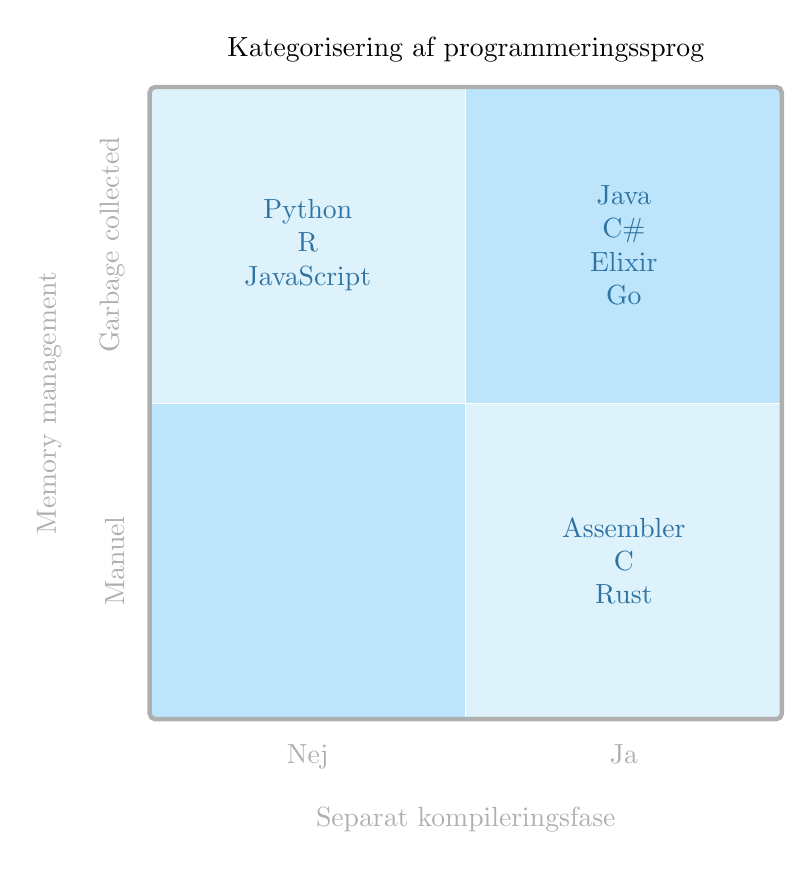
\begin{tikzpicture}[squares/.style={align=center, text width=3cm, text=bluetext, minimum width=4cm, minimum height=4cm}]

    \node[squares,fill=lightblue] (A) at (0,0) {Python\\R\\JavaScript};
    \node[squares,fill=darkblue,anchor=west] (B) at (A.east) {Java\\C\#\\Elixir\\Go};
    \node[squares,fill=darkblue,anchor=north] (C) at (A.south){};
    \node[squares,fill=lightblue,anchor=north] (D) at (B.south) {Assembler\\C\\Rust};
    \node[inner sep=0pt,draw=grey,ultra thick,rounded corners=2pt,fit=(A)(B)(C)(D)] {}; 

    \node[align=center,anchor=south,yshift=2mm] at (A.north east) {Kategorisering af programmeringssprog};
    \node[anchor=east,text=grey,xshift=-2mm] at (A.west) {\rotatebox{90}{Garbage collected}};
    \node[anchor=east,text=grey,xshift=-1cm,align=right] at (A.south west) {\rotatebox{90}{Memory management}};
    \node[anchor=east,text=grey,xshift=-2mm] at (C.west) {\rotatebox{90}{Manuel}};
    \node[anchor=north,text=grey,yshift=-2mm] at (C.south) {Nej};
    \node[anchor=north,text=grey,yshift=-1cm] at (C.south east) {Separat kompileringsfase};
    \node[anchor=north,text=grey,yshift=-2mm] at (D.south) {Ja};
\end{tikzpicture}


\section{Parsing}

% file content
Indholdet af en fil er en sekvens af bytes, altså værdier der hver især har én af 256 mulige værdier. Når vi skriver tekst fortolkes disse bytes som tegn og de programmer vi bruger til at åbne sådanne filer vælger at tegne hvert tegn til højre for det forrige. Ved linjebrud -- der repræsenteres ved en bestemt sekvens af tegn -- flyttes den horisontale position helt til venstre og der rykkes en linjehøjde nedaf. Nogle programmer bryder linjer der er for brede til ens skærm. Men det er sådan set det. En sådan tekstfil indeholder ikke nogen information om font eller tekststørrelse. Ønsker man at gemme sådanne informationer er man nødt til at introducere et \textsl{filformat}, der \textsl{koder} sådanne informationer ved sårlige opmærkninger. Men det er ikke relevant for filer der indeholder kode.

% human interpretation
Filer der indeholder kode er rå tekstfiler: En sekvens af tegn med linjebrud. Som programmører manipulerer vi disse filer igennem en teksteditor, der oftest -- ud over selve visningen af disse tegn -- vælger at farvekode udvalgte delsekvenser for at gøre teksten mere overskuelig for mennesker. Disse farver repræsenterer dog en \textsl{fortolkning} som værktøjet bruger til at berige koden. På samme måde er der nogen sådanne editorer der nummererer linjerne, fremhæver en aktuelle linje og markerer matchende parenteser.

% machine interpretation
Den tekst disse filer indeholder kaldes for \textsl{programkode} (eller blot \textsl{kode}), og vi ændrer i den på nogenlunde samme måde som vi ændrede i en dansk stil. Men når vi beder computeren om at køre noget med vores programkode så ser den filen på en anden måde. Indholdet er naturligvis det samme, men \textsl{fortolkningen} er anderledes: På baggrund af nogle regler opbygger computeren en træstruktur af programmet.

% TODO: træstruktur

\subsection{Regler}

% https://homepage.ruhr-uni-bochum.de/jan.holthuis/posts/using-the-latex-rail-package

\subsection{Parsetræer}

% https://tex.stackexchange.com/questions/111564/create-a-syntax-tree-with-latex

\chapter{Programmeringssprog}
\label{sec:lang}

\begin{inspiration}{Larry Wall}
Computer language design is just like a stroll in the park. Jurassic Park, that is.
\end{inspiration}

% inspiration: https://tex.stackexchange.com/questions/309425/how-is-it-possible-to-make-a-magic-quadrant
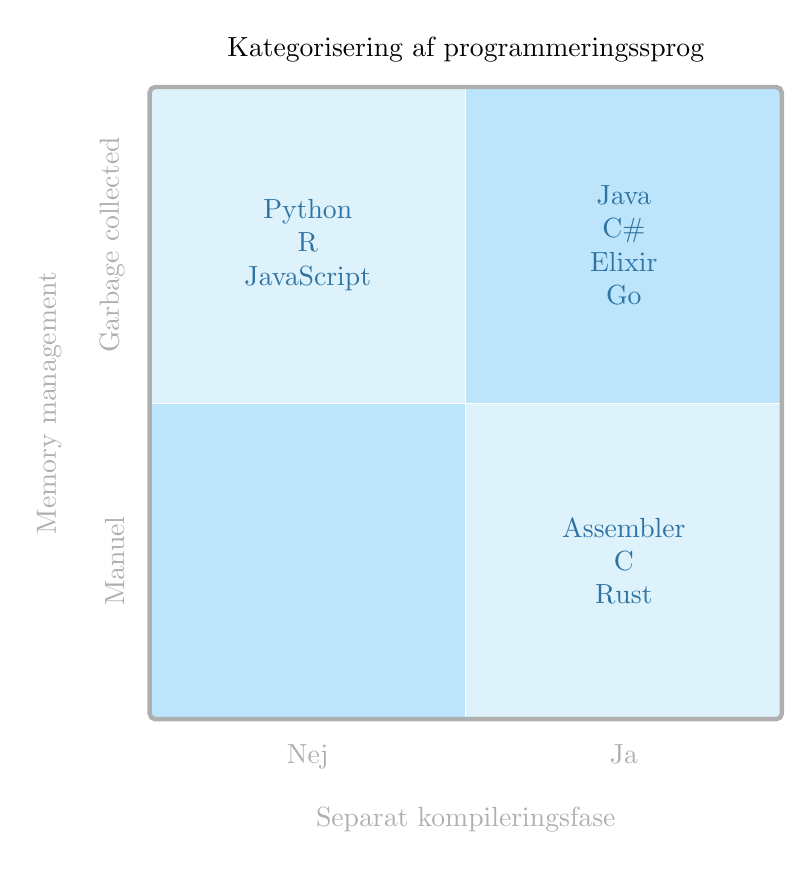
\begin{tikzpicture}[squares/.style={align=center, text width=3cm, text=bluetext, minimum width=4cm, minimum height=4cm}]

    \node[squares,fill=lightblue] (A) at (0,0) {Python\\R\\JavaScript};
    \node[squares,fill=darkblue,anchor=west] (B) at (A.east) {Java\\C\#\\Elixir\\Go};
    \node[squares,fill=darkblue,anchor=north] (C) at (A.south){};
    \node[squares,fill=lightblue,anchor=north] (D) at (B.south) {Assembler\\C\\Rust};
    \node[inner sep=0pt,draw=grey,ultra thick,rounded corners=2pt,fit=(A)(B)(C)(D)] {}; 

    \node[align=center,anchor=south,yshift=2mm] at (A.north east) {Kategorisering af programmeringssprog};
    \node[anchor=east,text=grey,xshift=-2mm] at (A.west) {\rotatebox{90}{Garbage collected}};
    \node[anchor=east,text=grey,xshift=-1cm,align=right] at (A.south west) {\rotatebox{90}{Memory management}};
    \node[anchor=east,text=grey,xshift=-2mm] at (C.west) {\rotatebox{90}{Manuel}};
    \node[anchor=north,text=grey,yshift=-2mm] at (C.south) {Nej};
    \node[anchor=north,text=grey,yshift=-1cm] at (C.south east) {Separat kompileringsfase};
    \node[anchor=north,text=grey,yshift=-2mm] at (D.south) {Ja};
\end{tikzpicture}


\section{Parsing}

% file content
Indholdet af en fil er en sekvens af bytes, altså værdier der hver især har én af 256 mulige værdier. Når vi skriver tekst fortolkes disse bytes som tegn og de programmer vi bruger til at åbne sådanne filer vælger at tegne hvert tegn til højre for det forrige. Ved linjebrud -- der repræsenteres ved en bestemt sekvens af tegn -- flyttes den horisontale position helt til venstre og der rykkes en linjehøjde nedaf. Nogle programmer bryder linjer der er for brede til ens skærm. Men det er sådan set det. En sådan tekstfil indeholder ikke nogen information om font eller tekststørrelse. Ønsker man at gemme sådanne informationer er man nødt til at introducere et \textsl{filformat}, der \textsl{koder} sådanne informationer ved sårlige opmærkninger. Men det er ikke relevant for filer der indeholder kode.

% human interpretation
Filer der indeholder kode er rå tekstfiler: En sekvens af tegn med linjebrud. Som programmører manipulerer vi disse filer igennem en teksteditor, der oftest -- ud over selve visningen af disse tegn -- vælger at farvekode udvalgte delsekvenser for at gøre teksten mere overskuelig for mennesker. Disse farver repræsenterer dog en \textsl{fortolkning} som værktøjet bruger til at berige koden. På samme måde er der nogen sådanne editorer der nummererer linjerne, fremhæver en aktuelle linje og markerer matchende parenteser.

% machine interpretation
Den tekst disse filer indeholder kaldes for \textsl{programkode} (eller blot \textsl{kode}), og vi ændrer i den på nogenlunde samme måde som vi ændrede i en dansk stil. Men når vi beder computeren om at køre noget med vores programkode så ser den filen på en anden måde. Indholdet er naturligvis det samme, men \textsl{fortolkningen} er anderledes: På baggrund af nogle regler opbygger computeren en træstruktur af programmet.

% TODO: træstruktur

\subsection{Regler}

% https://homepage.ruhr-uni-bochum.de/jan.holthuis/posts/using-the-latex-rail-package

\subsection{Parsetræer}

% https://tex.stackexchange.com/questions/111564/create-a-syntax-tree-with-latex

\chapter{Programmeringssprog}
\label{sec:lang}

\begin{inspiration}{Larry Wall}
Computer language design is just like a stroll in the park. Jurassic Park, that is.
\end{inspiration}

% inspiration: https://tex.stackexchange.com/questions/309425/how-is-it-possible-to-make-a-magic-quadrant
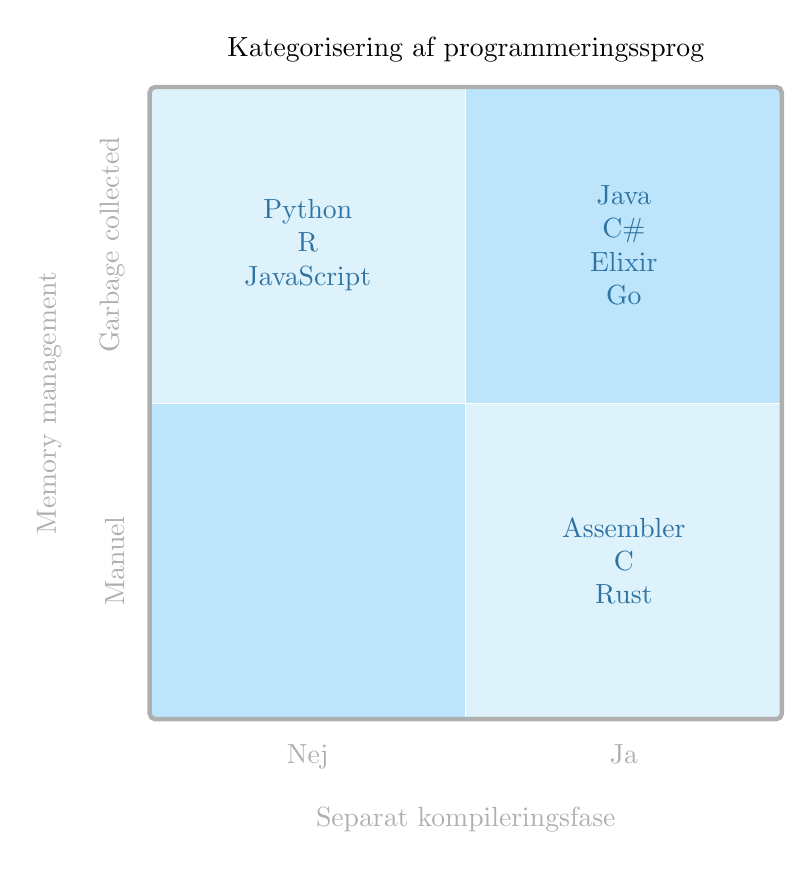
\begin{tikzpicture}[squares/.style={align=center, text width=3cm, text=bluetext, minimum width=4cm, minimum height=4cm}]

    \node[squares,fill=lightblue] (A) at (0,0) {Python\\R\\JavaScript};
    \node[squares,fill=darkblue,anchor=west] (B) at (A.east) {Java\\C\#\\Elixir\\Go};
    \node[squares,fill=darkblue,anchor=north] (C) at (A.south){};
    \node[squares,fill=lightblue,anchor=north] (D) at (B.south) {Assembler\\C\\Rust};
    \node[inner sep=0pt,draw=grey,ultra thick,rounded corners=2pt,fit=(A)(B)(C)(D)] {}; 

    \node[align=center,anchor=south,yshift=2mm] at (A.north east) {Kategorisering af programmeringssprog};
    \node[anchor=east,text=grey,xshift=-2mm] at (A.west) {\rotatebox{90}{Garbage collected}};
    \node[anchor=east,text=grey,xshift=-1cm,align=right] at (A.south west) {\rotatebox{90}{Memory management}};
    \node[anchor=east,text=grey,xshift=-2mm] at (C.west) {\rotatebox{90}{Manuel}};
    \node[anchor=north,text=grey,yshift=-2mm] at (C.south) {Nej};
    \node[anchor=north,text=grey,yshift=-1cm] at (C.south east) {Separat kompileringsfase};
    \node[anchor=north,text=grey,yshift=-2mm] at (D.south) {Ja};
\end{tikzpicture}


\section{Parsing}

% file content
Indholdet af en fil er en sekvens af bytes, altså værdier der hver især har én af 256 mulige værdier. Når vi skriver tekst fortolkes disse bytes som tegn og de programmer vi bruger til at åbne sådanne filer vælger at tegne hvert tegn til højre for det forrige. Ved linjebrud -- der repræsenteres ved en bestemt sekvens af tegn -- flyttes den horisontale position helt til venstre og der rykkes en linjehøjde nedaf. Nogle programmer bryder linjer der er for brede til ens skærm. Men det er sådan set det. En sådan tekstfil indeholder ikke nogen information om font eller tekststørrelse. Ønsker man at gemme sådanne informationer er man nødt til at introducere et \textsl{filformat}, der \textsl{koder} sådanne informationer ved sårlige opmærkninger. Men det er ikke relevant for filer der indeholder kode.

% human interpretation
Filer der indeholder kode er rå tekstfiler: En sekvens af tegn med linjebrud. Som programmører manipulerer vi disse filer igennem en teksteditor, der oftest -- ud over selve visningen af disse tegn -- vælger at farvekode udvalgte delsekvenser for at gøre teksten mere overskuelig for mennesker. Disse farver repræsenterer dog en \textsl{fortolkning} som værktøjet bruger til at berige koden. På samme måde er der nogen sådanne editorer der nummererer linjerne, fremhæver en aktuelle linje og markerer matchende parenteser.

% machine interpretation
Den tekst disse filer indeholder kaldes for \textsl{programkode} (eller blot \textsl{kode}), og vi ændrer i den på nogenlunde samme måde som vi ændrede i en dansk stil. Men når vi beder computeren om at køre noget med vores programkode så ser den filen på en anden måde. Indholdet er naturligvis det samme, men \textsl{fortolkningen} er anderledes: På baggrund af nogle regler opbygger computeren en træstruktur af programmet.

% TODO: træstruktur

\subsection{Regler}

% https://homepage.ruhr-uni-bochum.de/jan.holthuis/posts/using-the-latex-rail-package

\subsection{Parsetræer}

% https://tex.stackexchange.com/questions/111564/create-a-syntax-tree-with-latex

\chapter{Programmeringssprog}
\label{sec:lang}

\begin{inspiration}{Larry Wall}
Computer language design is just like a stroll in the park. Jurassic Park, that is.
\end{inspiration}

% inspiration: https://tex.stackexchange.com/questions/309425/how-is-it-possible-to-make-a-magic-quadrant
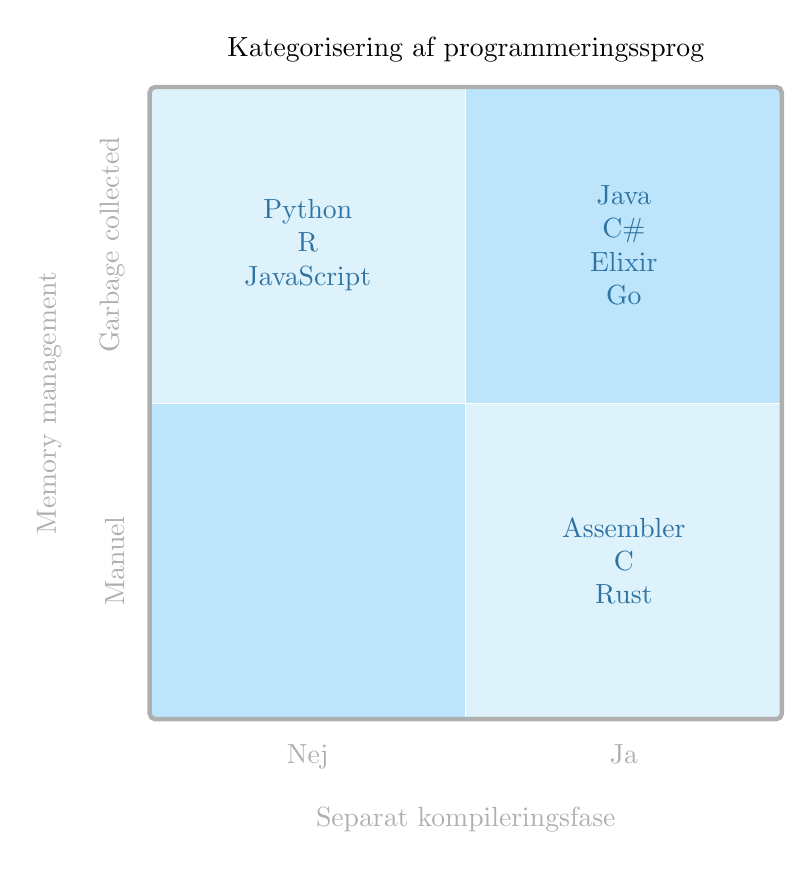
\begin{tikzpicture}[squares/.style={align=center, text width=3cm, text=bluetext, minimum width=4cm, minimum height=4cm}]

    \node[squares,fill=lightblue] (A) at (0,0) {Python\\R\\JavaScript};
    \node[squares,fill=darkblue,anchor=west] (B) at (A.east) {Java\\C\#\\Elixir\\Go};
    \node[squares,fill=darkblue,anchor=north] (C) at (A.south){};
    \node[squares,fill=lightblue,anchor=north] (D) at (B.south) {Assembler\\C\\Rust};
    \node[inner sep=0pt,draw=grey,ultra thick,rounded corners=2pt,fit=(A)(B)(C)(D)] {}; 

    \node[align=center,anchor=south,yshift=2mm] at (A.north east) {Kategorisering af programmeringssprog};
    \node[anchor=east,text=grey,xshift=-2mm] at (A.west) {\rotatebox{90}{Garbage collected}};
    \node[anchor=east,text=grey,xshift=-1cm,align=right] at (A.south west) {\rotatebox{90}{Memory management}};
    \node[anchor=east,text=grey,xshift=-2mm] at (C.west) {\rotatebox{90}{Manuel}};
    \node[anchor=north,text=grey,yshift=-2mm] at (C.south) {Nej};
    \node[anchor=north,text=grey,yshift=-1cm] at (C.south east) {Separat kompileringsfase};
    \node[anchor=north,text=grey,yshift=-2mm] at (D.south) {Ja};
\end{tikzpicture}


\section{Parsing}

% file content
Indholdet af en fil er en sekvens af bytes, altså værdier der hver især har én af 256 mulige værdier. Når vi skriver tekst fortolkes disse bytes som tegn og de programmer vi bruger til at åbne sådanne filer vælger at tegne hvert tegn til højre for det forrige. Ved linjebrud -- der repræsenteres ved en bestemt sekvens af tegn -- flyttes den horisontale position helt til venstre og der rykkes en linjehøjde nedaf. Nogle programmer bryder linjer der er for brede til ens skærm. Men det er sådan set det. En sådan tekstfil indeholder ikke nogen information om font eller tekststørrelse. Ønsker man at gemme sådanne informationer er man nødt til at introducere et \textsl{filformat}, der \textsl{koder} sådanne informationer ved sårlige opmærkninger. Men det er ikke relevant for filer der indeholder kode.

% human interpretation
Filer der indeholder kode er rå tekstfiler: En sekvens af tegn med linjebrud. Som programmører manipulerer vi disse filer igennem en teksteditor, der oftest -- ud over selve visningen af disse tegn -- vælger at farvekode udvalgte delsekvenser for at gøre teksten mere overskuelig for mennesker. Disse farver repræsenterer dog en \textsl{fortolkning} som værktøjet bruger til at berige koden. På samme måde er der nogen sådanne editorer der nummererer linjerne, fremhæver en aktuelle linje og markerer matchende parenteser.

% machine interpretation
Den tekst disse filer indeholder kaldes for \textsl{programkode} (eller blot \textsl{kode}), og vi ændrer i den på nogenlunde samme måde som vi ændrede i en dansk stil. Men når vi beder computeren om at køre noget med vores programkode så ser den filen på en anden måde. Indholdet er naturligvis det samme, men \textsl{fortolkningen} er anderledes: På baggrund af nogle regler opbygger computeren en træstruktur af programmet.

% TODO: træstruktur

\subsection{Regler}

% https://homepage.ruhr-uni-bochum.de/jan.holthuis/posts/using-the-latex-rail-package

\subsection{Parsetræer}

% https://tex.stackexchange.com/questions/111564/create-a-syntax-tree-with-latex

\chapter{Programmeringssprog}
\label{sec:lang}

\begin{inspiration}{Larry Wall}
Computer language design is just like a stroll in the park. Jurassic Park, that is.
\end{inspiration}

% inspiration: https://tex.stackexchange.com/questions/309425/how-is-it-possible-to-make-a-magic-quadrant
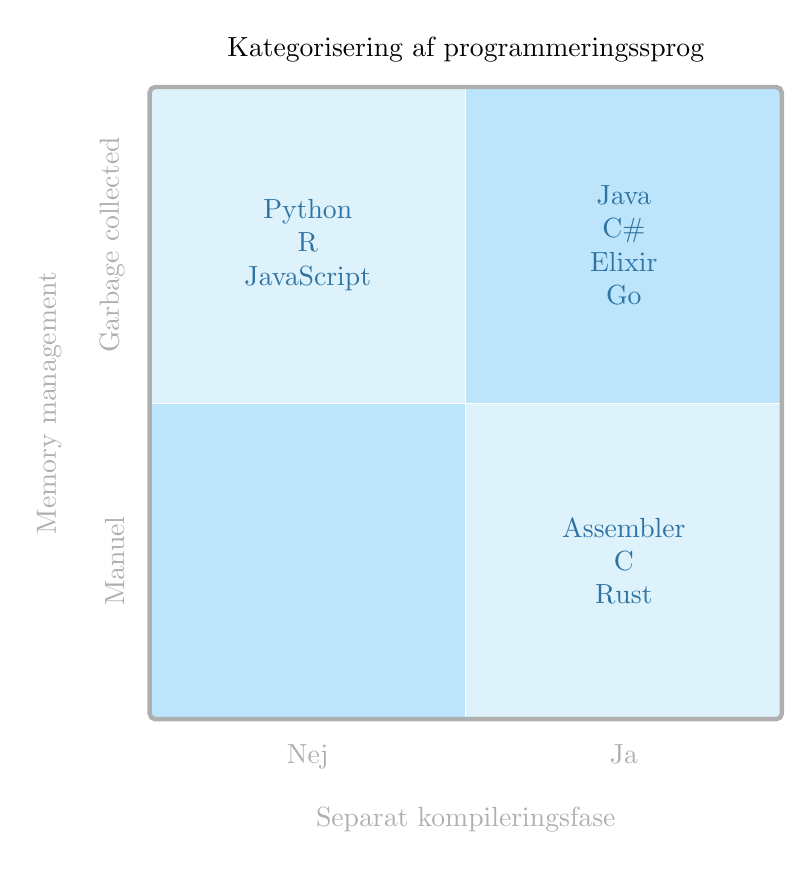
\begin{tikzpicture}[squares/.style={align=center, text width=3cm, text=bluetext, minimum width=4cm, minimum height=4cm}]

    \node[squares,fill=lightblue] (A) at (0,0) {Python\\R\\JavaScript};
    \node[squares,fill=darkblue,anchor=west] (B) at (A.east) {Java\\C\#\\Elixir\\Go};
    \node[squares,fill=darkblue,anchor=north] (C) at (A.south){};
    \node[squares,fill=lightblue,anchor=north] (D) at (B.south) {Assembler\\C\\Rust};
    \node[inner sep=0pt,draw=grey,ultra thick,rounded corners=2pt,fit=(A)(B)(C)(D)] {}; 

    \node[align=center,anchor=south,yshift=2mm] at (A.north east) {Kategorisering af programmeringssprog};
    \node[anchor=east,text=grey,xshift=-2mm] at (A.west) {\rotatebox{90}{Garbage collected}};
    \node[anchor=east,text=grey,xshift=-1cm,align=right] at (A.south west) {\rotatebox{90}{Memory management}};
    \node[anchor=east,text=grey,xshift=-2mm] at (C.west) {\rotatebox{90}{Manuel}};
    \node[anchor=north,text=grey,yshift=-2mm] at (C.south) {Nej};
    \node[anchor=north,text=grey,yshift=-1cm] at (C.south east) {Separat kompileringsfase};
    \node[anchor=north,text=grey,yshift=-2mm] at (D.south) {Ja};
\end{tikzpicture}


\section{Parsing}

% file content
Indholdet af en fil er en sekvens af bytes, altså værdier der hver især har én af 256 mulige værdier. Når vi skriver tekst fortolkes disse bytes som tegn og de programmer vi bruger til at åbne sådanne filer vælger at tegne hvert tegn til højre for det forrige. Ved linjebrud -- der repræsenteres ved en bestemt sekvens af tegn -- flyttes den horisontale position helt til venstre og der rykkes en linjehøjde nedaf. Nogle programmer bryder linjer der er for brede til ens skærm. Men det er sådan set det. En sådan tekstfil indeholder ikke nogen information om font eller tekststørrelse. Ønsker man at gemme sådanne informationer er man nødt til at introducere et \textsl{filformat}, der \textsl{koder} sådanne informationer ved sårlige opmærkninger. Men det er ikke relevant for filer der indeholder kode.

% human interpretation
Filer der indeholder kode er rå tekstfiler: En sekvens af tegn med linjebrud. Som programmører manipulerer vi disse filer igennem en teksteditor, der oftest -- ud over selve visningen af disse tegn -- vælger at farvekode udvalgte delsekvenser for at gøre teksten mere overskuelig for mennesker. Disse farver repræsenterer dog en \textsl{fortolkning} som værktøjet bruger til at berige koden. På samme måde er der nogen sådanne editorer der nummererer linjerne, fremhæver en aktuelle linje og markerer matchende parenteser.

% machine interpretation
Den tekst disse filer indeholder kaldes for \textsl{programkode} (eller blot \textsl{kode}), og vi ændrer i den på nogenlunde samme måde som vi ændrede i en dansk stil. Men når vi beder computeren om at køre noget med vores programkode så ser den filen på en anden måde. Indholdet er naturligvis det samme, men \textsl{fortolkningen} er anderledes: På baggrund af nogle regler opbygger computeren en træstruktur af programmet.

% TODO: træstruktur

\subsection{Regler}

% https://homepage.ruhr-uni-bochum.de/jan.holthuis/posts/using-the-latex-rail-package

\subsection{Parsetræer}

% https://tex.stackexchange.com/questions/111564/create-a-syntax-tree-with-latex

\chapter{Programmeringssprog}
\label{sec:lang}

\begin{inspiration}{Larry Wall}
Computer language design is just like a stroll in the park. Jurassic Park, that is.
\end{inspiration}

% inspiration: https://tex.stackexchange.com/questions/309425/how-is-it-possible-to-make-a-magic-quadrant
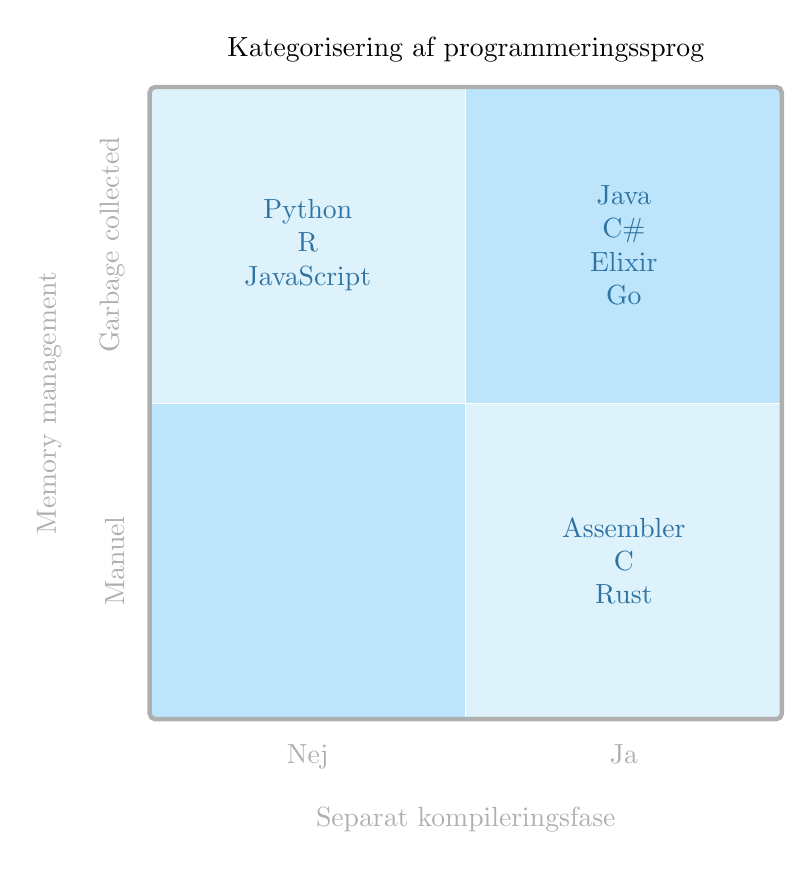
\begin{tikzpicture}[squares/.style={align=center, text width=3cm, text=bluetext, minimum width=4cm, minimum height=4cm}]

    \node[squares,fill=lightblue] (A) at (0,0) {Python\\R\\JavaScript};
    \node[squares,fill=darkblue,anchor=west] (B) at (A.east) {Java\\C\#\\Elixir\\Go};
    \node[squares,fill=darkblue,anchor=north] (C) at (A.south){};
    \node[squares,fill=lightblue,anchor=north] (D) at (B.south) {Assembler\\C\\Rust};
    \node[inner sep=0pt,draw=grey,ultra thick,rounded corners=2pt,fit=(A)(B)(C)(D)] {}; 

    \node[align=center,anchor=south,yshift=2mm] at (A.north east) {Kategorisering af programmeringssprog};
    \node[anchor=east,text=grey,xshift=-2mm] at (A.west) {\rotatebox{90}{Garbage collected}};
    \node[anchor=east,text=grey,xshift=-1cm,align=right] at (A.south west) {\rotatebox{90}{Memory management}};
    \node[anchor=east,text=grey,xshift=-2mm] at (C.west) {\rotatebox{90}{Manuel}};
    \node[anchor=north,text=grey,yshift=-2mm] at (C.south) {Nej};
    \node[anchor=north,text=grey,yshift=-1cm] at (C.south east) {Separat kompileringsfase};
    \node[anchor=north,text=grey,yshift=-2mm] at (D.south) {Ja};
\end{tikzpicture}


\section{Parsing}

% file content
Indholdet af en fil er en sekvens af bytes, altså værdier der hver især har én af 256 mulige værdier. Når vi skriver tekst fortolkes disse bytes som tegn og de programmer vi bruger til at åbne sådanne filer vælger at tegne hvert tegn til højre for det forrige. Ved linjebrud -- der repræsenteres ved en bestemt sekvens af tegn -- flyttes den horisontale position helt til venstre og der rykkes en linjehøjde nedaf. Nogle programmer bryder linjer der er for brede til ens skærm. Men det er sådan set det. En sådan tekstfil indeholder ikke nogen information om font eller tekststørrelse. Ønsker man at gemme sådanne informationer er man nødt til at introducere et \textsl{filformat}, der \textsl{koder} sådanne informationer ved sårlige opmærkninger. Men det er ikke relevant for filer der indeholder kode.

% human interpretation
Filer der indeholder kode er rå tekstfiler: En sekvens af tegn med linjebrud. Som programmører manipulerer vi disse filer igennem en teksteditor, der oftest -- ud over selve visningen af disse tegn -- vælger at farvekode udvalgte delsekvenser for at gøre teksten mere overskuelig for mennesker. Disse farver repræsenterer dog en \textsl{fortolkning} som værktøjet bruger til at berige koden. På samme måde er der nogen sådanne editorer der nummererer linjerne, fremhæver en aktuelle linje og markerer matchende parenteser.

% machine interpretation
Den tekst disse filer indeholder kaldes for \textsl{programkode} (eller blot \textsl{kode}), og vi ændrer i den på nogenlunde samme måde som vi ændrede i en dansk stil. Men når vi beder computeren om at køre noget med vores programkode så ser den filen på en anden måde. Indholdet er naturligvis det samme, men \textsl{fortolkningen} er anderledes: På baggrund af nogle regler opbygger computeren en træstruktur af programmet.

% TODO: træstruktur

\subsection{Regler}

% https://homepage.ruhr-uni-bochum.de/jan.holthuis/posts/using-the-latex-rail-package

\subsection{Parsetræer}

% https://tex.stackexchange.com/questions/111564/create-a-syntax-tree-with-latex

\chapter{Programmeringssprog}
\label{sec:lang}

\begin{inspiration}{Larry Wall}
Computer language design is just like a stroll in the park. Jurassic Park, that is.
\end{inspiration}

% inspiration: https://tex.stackexchange.com/questions/309425/how-is-it-possible-to-make-a-magic-quadrant
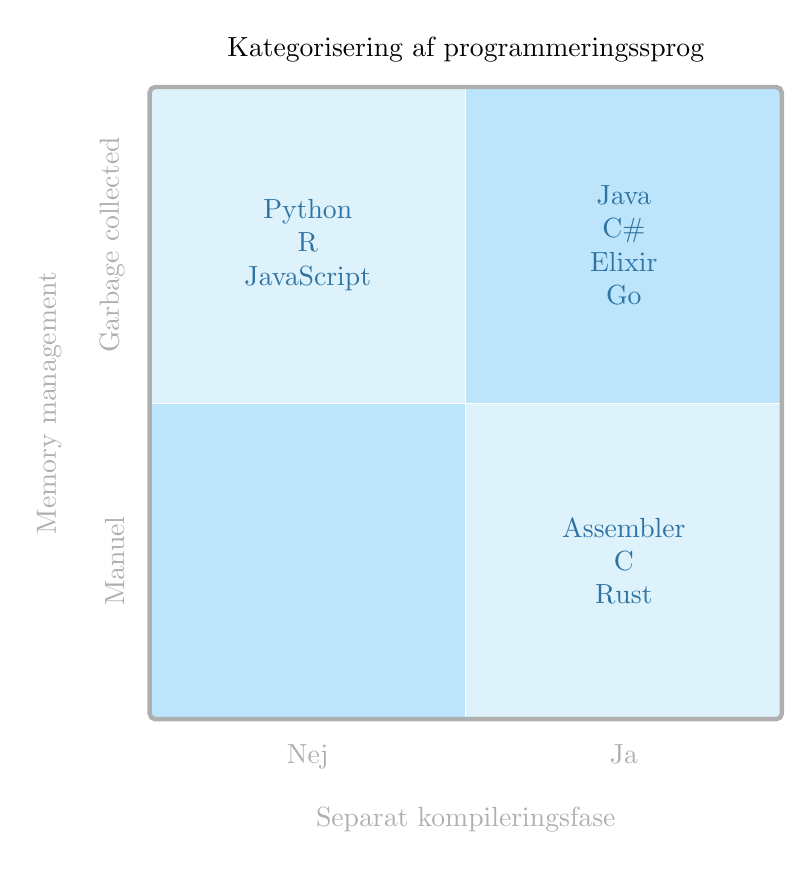
\begin{tikzpicture}[squares/.style={align=center, text width=3cm, text=bluetext, minimum width=4cm, minimum height=4cm}]

    \node[squares,fill=lightblue] (A) at (0,0) {Python\\R\\JavaScript};
    \node[squares,fill=darkblue,anchor=west] (B) at (A.east) {Java\\C\#\\Elixir\\Go};
    \node[squares,fill=darkblue,anchor=north] (C) at (A.south){};
    \node[squares,fill=lightblue,anchor=north] (D) at (B.south) {Assembler\\C\\Rust};
    \node[inner sep=0pt,draw=grey,ultra thick,rounded corners=2pt,fit=(A)(B)(C)(D)] {}; 

    \node[align=center,anchor=south,yshift=2mm] at (A.north east) {Kategorisering af programmeringssprog};
    \node[anchor=east,text=grey,xshift=-2mm] at (A.west) {\rotatebox{90}{Garbage collected}};
    \node[anchor=east,text=grey,xshift=-1cm,align=right] at (A.south west) {\rotatebox{90}{Memory management}};
    \node[anchor=east,text=grey,xshift=-2mm] at (C.west) {\rotatebox{90}{Manuel}};
    \node[anchor=north,text=grey,yshift=-2mm] at (C.south) {Nej};
    \node[anchor=north,text=grey,yshift=-1cm] at (C.south east) {Separat kompileringsfase};
    \node[anchor=north,text=grey,yshift=-2mm] at (D.south) {Ja};
\end{tikzpicture}


\section{Parsing}

% file content
Indholdet af en fil er en sekvens af bytes, altså værdier der hver især har én af 256 mulige værdier. Når vi skriver tekst fortolkes disse bytes som tegn og de programmer vi bruger til at åbne sådanne filer vælger at tegne hvert tegn til højre for det forrige. Ved linjebrud -- der repræsenteres ved en bestemt sekvens af tegn -- flyttes den horisontale position helt til venstre og der rykkes en linjehøjde nedaf. Nogle programmer bryder linjer der er for brede til ens skærm. Men det er sådan set det. En sådan tekstfil indeholder ikke nogen information om font eller tekststørrelse. Ønsker man at gemme sådanne informationer er man nødt til at introducere et \textsl{filformat}, der \textsl{koder} sådanne informationer ved sårlige opmærkninger. Men det er ikke relevant for filer der indeholder kode.

% human interpretation
Filer der indeholder kode er rå tekstfiler: En sekvens af tegn med linjebrud. Som programmører manipulerer vi disse filer igennem en teksteditor, der oftest -- ud over selve visningen af disse tegn -- vælger at farvekode udvalgte delsekvenser for at gøre teksten mere overskuelig for mennesker. Disse farver repræsenterer dog en \textsl{fortolkning} som værktøjet bruger til at berige koden. På samme måde er der nogen sådanne editorer der nummererer linjerne, fremhæver en aktuelle linje og markerer matchende parenteser.

% machine interpretation
Den tekst disse filer indeholder kaldes for \textsl{programkode} (eller blot \textsl{kode}), og vi ændrer i den på nogenlunde samme måde som vi ændrede i en dansk stil. Men når vi beder computeren om at køre noget med vores programkode så ser den filen på en anden måde. Indholdet er naturligvis det samme, men \textsl{fortolkningen} er anderledes: På baggrund af nogle regler opbygger computeren en træstruktur af programmet.

% TODO: træstruktur

\subsection{Regler}

% https://homepage.ruhr-uni-bochum.de/jan.holthuis/posts/using-the-latex-rail-package

\subsection{Parsetræer}

% https://tex.stackexchange.com/questions/111564/create-a-syntax-tree-with-latex

\chapter{Programmeringssprog}
\label{sec:lang}

\begin{inspiration}{Larry Wall}
Computer language design is just like a stroll in the park. Jurassic Park, that is.
\end{inspiration}

% inspiration: https://tex.stackexchange.com/questions/309425/how-is-it-possible-to-make-a-magic-quadrant
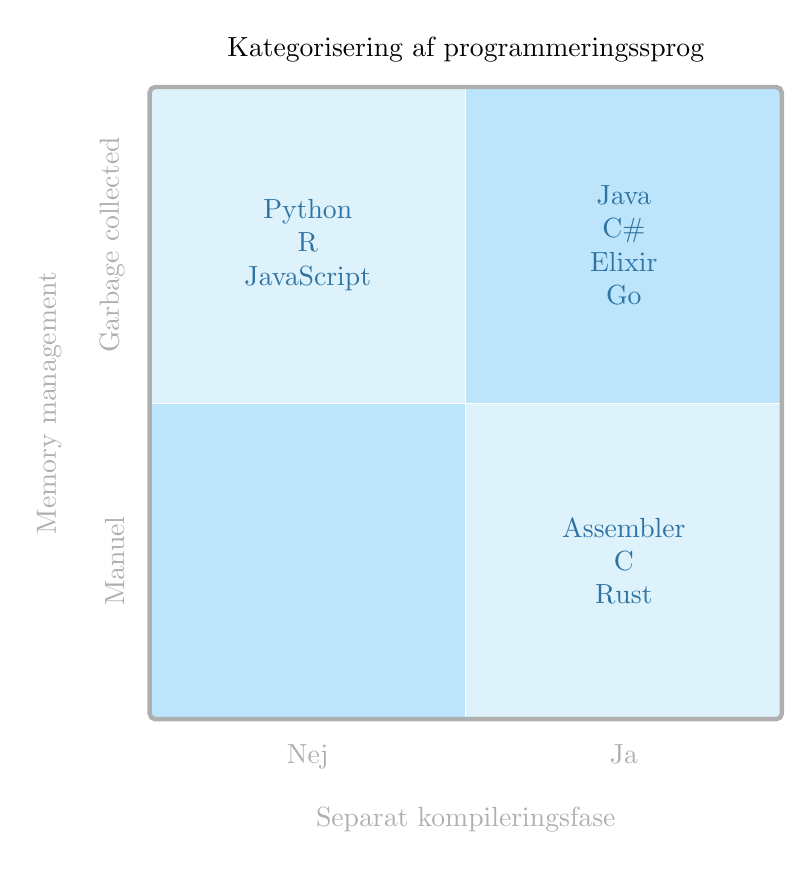
\begin{tikzpicture}[squares/.style={align=center, text width=3cm, text=bluetext, minimum width=4cm, minimum height=4cm}]

    \node[squares,fill=lightblue] (A) at (0,0) {Python\\R\\JavaScript};
    \node[squares,fill=darkblue,anchor=west] (B) at (A.east) {Java\\C\#\\Elixir\\Go};
    \node[squares,fill=darkblue,anchor=north] (C) at (A.south){};
    \node[squares,fill=lightblue,anchor=north] (D) at (B.south) {Assembler\\C\\Rust};
    \node[inner sep=0pt,draw=grey,ultra thick,rounded corners=2pt,fit=(A)(B)(C)(D)] {}; 

    \node[align=center,anchor=south,yshift=2mm] at (A.north east) {Kategorisering af programmeringssprog};
    \node[anchor=east,text=grey,xshift=-2mm] at (A.west) {\rotatebox{90}{Garbage collected}};
    \node[anchor=east,text=grey,xshift=-1cm,align=right] at (A.south west) {\rotatebox{90}{Memory management}};
    \node[anchor=east,text=grey,xshift=-2mm] at (C.west) {\rotatebox{90}{Manuel}};
    \node[anchor=north,text=grey,yshift=-2mm] at (C.south) {Nej};
    \node[anchor=north,text=grey,yshift=-1cm] at (C.south east) {Separat kompileringsfase};
    \node[anchor=north,text=grey,yshift=-2mm] at (D.south) {Ja};
\end{tikzpicture}


\section{Parsing}

% file content
Indholdet af en fil er en sekvens af bytes, altså værdier der hver især har én af 256 mulige værdier. Når vi skriver tekst fortolkes disse bytes som tegn og de programmer vi bruger til at åbne sådanne filer vælger at tegne hvert tegn til højre for det forrige. Ved linjebrud -- der repræsenteres ved en bestemt sekvens af tegn -- flyttes den horisontale position helt til venstre og der rykkes en linjehøjde nedaf. Nogle programmer bryder linjer der er for brede til ens skærm. Men det er sådan set det. En sådan tekstfil indeholder ikke nogen information om font eller tekststørrelse. Ønsker man at gemme sådanne informationer er man nødt til at introducere et \textsl{filformat}, der \textsl{koder} sådanne informationer ved sårlige opmærkninger. Men det er ikke relevant for filer der indeholder kode.

% human interpretation
Filer der indeholder kode er rå tekstfiler: En sekvens af tegn med linjebrud. Som programmører manipulerer vi disse filer igennem en teksteditor, der oftest -- ud over selve visningen af disse tegn -- vælger at farvekode udvalgte delsekvenser for at gøre teksten mere overskuelig for mennesker. Disse farver repræsenterer dog en \textsl{fortolkning} som værktøjet bruger til at berige koden. På samme måde er der nogen sådanne editorer der nummererer linjerne, fremhæver en aktuelle linje og markerer matchende parenteser.

% machine interpretation
Den tekst disse filer indeholder kaldes for \textsl{programkode} (eller blot \textsl{kode}), og vi ændrer i den på nogenlunde samme måde som vi ændrede i en dansk stil. Men når vi beder computeren om at køre noget med vores programkode så ser den filen på en anden måde. Indholdet er naturligvis det samme, men \textsl{fortolkningen} er anderledes: På baggrund af nogle regler opbygger computeren en træstruktur af programmet.

% TODO: træstruktur

\subsection{Regler}

% https://homepage.ruhr-uni-bochum.de/jan.holthuis/posts/using-the-latex-rail-package

\subsection{Parsetræer}

% https://tex.stackexchange.com/questions/111564/create-a-syntax-tree-with-latex

\chapter{Programmeringssprog}
\label{sec:lang}

\begin{inspiration}{Larry Wall}
Computer language design is just like a stroll in the park. Jurassic Park, that is.
\end{inspiration}

% inspiration: https://tex.stackexchange.com/questions/309425/how-is-it-possible-to-make-a-magic-quadrant
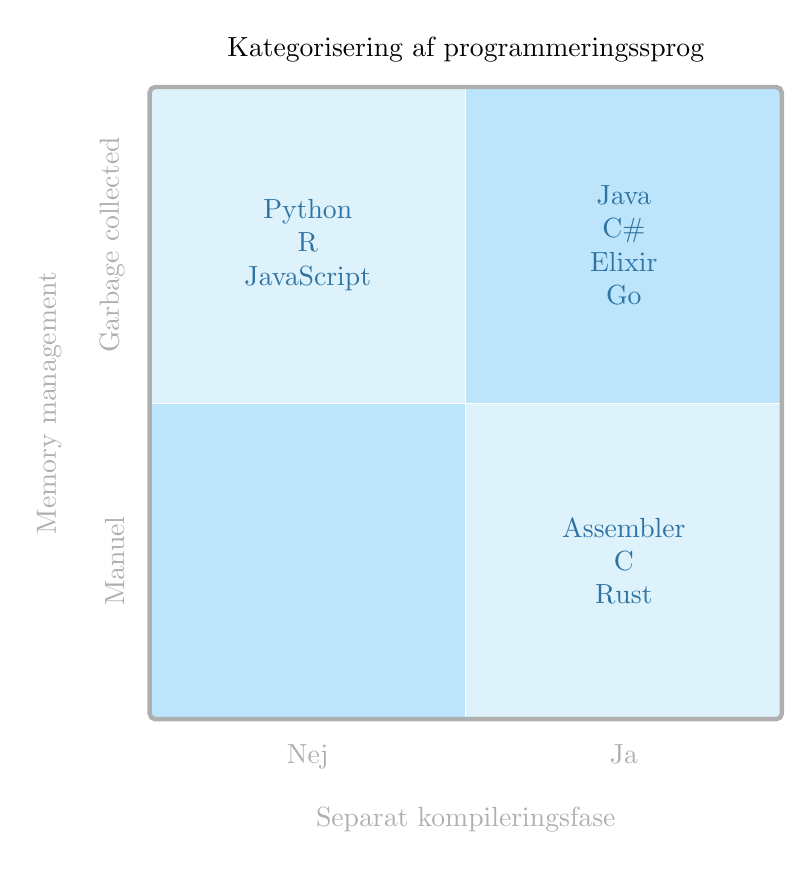
\begin{tikzpicture}[squares/.style={align=center, text width=3cm, text=bluetext, minimum width=4cm, minimum height=4cm}]

    \node[squares,fill=lightblue] (A) at (0,0) {Python\\R\\JavaScript};
    \node[squares,fill=darkblue,anchor=west] (B) at (A.east) {Java\\C\#\\Elixir\\Go};
    \node[squares,fill=darkblue,anchor=north] (C) at (A.south){};
    \node[squares,fill=lightblue,anchor=north] (D) at (B.south) {Assembler\\C\\Rust};
    \node[inner sep=0pt,draw=grey,ultra thick,rounded corners=2pt,fit=(A)(B)(C)(D)] {}; 

    \node[align=center,anchor=south,yshift=2mm] at (A.north east) {Kategorisering af programmeringssprog};
    \node[anchor=east,text=grey,xshift=-2mm] at (A.west) {\rotatebox{90}{Garbage collected}};
    \node[anchor=east,text=grey,xshift=-1cm,align=right] at (A.south west) {\rotatebox{90}{Memory management}};
    \node[anchor=east,text=grey,xshift=-2mm] at (C.west) {\rotatebox{90}{Manuel}};
    \node[anchor=north,text=grey,yshift=-2mm] at (C.south) {Nej};
    \node[anchor=north,text=grey,yshift=-1cm] at (C.south east) {Separat kompileringsfase};
    \node[anchor=north,text=grey,yshift=-2mm] at (D.south) {Ja};
\end{tikzpicture}


\section{Parsing}

% file content
Indholdet af en fil er en sekvens af bytes, altså værdier der hver især har én af 256 mulige værdier. Når vi skriver tekst fortolkes disse bytes som tegn og de programmer vi bruger til at åbne sådanne filer vælger at tegne hvert tegn til højre for det forrige. Ved linjebrud -- der repræsenteres ved en bestemt sekvens af tegn -- flyttes den horisontale position helt til venstre og der rykkes en linjehøjde nedaf. Nogle programmer bryder linjer der er for brede til ens skærm. Men det er sådan set det. En sådan tekstfil indeholder ikke nogen information om font eller tekststørrelse. Ønsker man at gemme sådanne informationer er man nødt til at introducere et \textsl{filformat}, der \textsl{koder} sådanne informationer ved sårlige opmærkninger. Men det er ikke relevant for filer der indeholder kode.

% human interpretation
Filer der indeholder kode er rå tekstfiler: En sekvens af tegn med linjebrud. Som programmører manipulerer vi disse filer igennem en teksteditor, der oftest -- ud over selve visningen af disse tegn -- vælger at farvekode udvalgte delsekvenser for at gøre teksten mere overskuelig for mennesker. Disse farver repræsenterer dog en \textsl{fortolkning} som værktøjet bruger til at berige koden. På samme måde er der nogen sådanne editorer der nummererer linjerne, fremhæver en aktuelle linje og markerer matchende parenteser.

% machine interpretation
Den tekst disse filer indeholder kaldes for \textsl{programkode} (eller blot \textsl{kode}), og vi ændrer i den på nogenlunde samme måde som vi ændrede i en dansk stil. Men når vi beder computeren om at køre noget med vores programkode så ser den filen på en anden måde. Indholdet er naturligvis det samme, men \textsl{fortolkningen} er anderledes: På baggrund af nogle regler opbygger computeren en træstruktur af programmet.

% TODO: træstruktur

\subsection{Regler}

% https://homepage.ruhr-uni-bochum.de/jan.holthuis/posts/using-the-latex-rail-package

\subsection{Parsetræer}

% https://tex.stackexchange.com/questions/111564/create-a-syntax-tree-with-latex

\chapter{Programmeringssprog}
\label{sec:lang}

\begin{inspiration}{Larry Wall}
Computer language design is just like a stroll in the park. Jurassic Park, that is.
\end{inspiration}

% inspiration: https://tex.stackexchange.com/questions/309425/how-is-it-possible-to-make-a-magic-quadrant
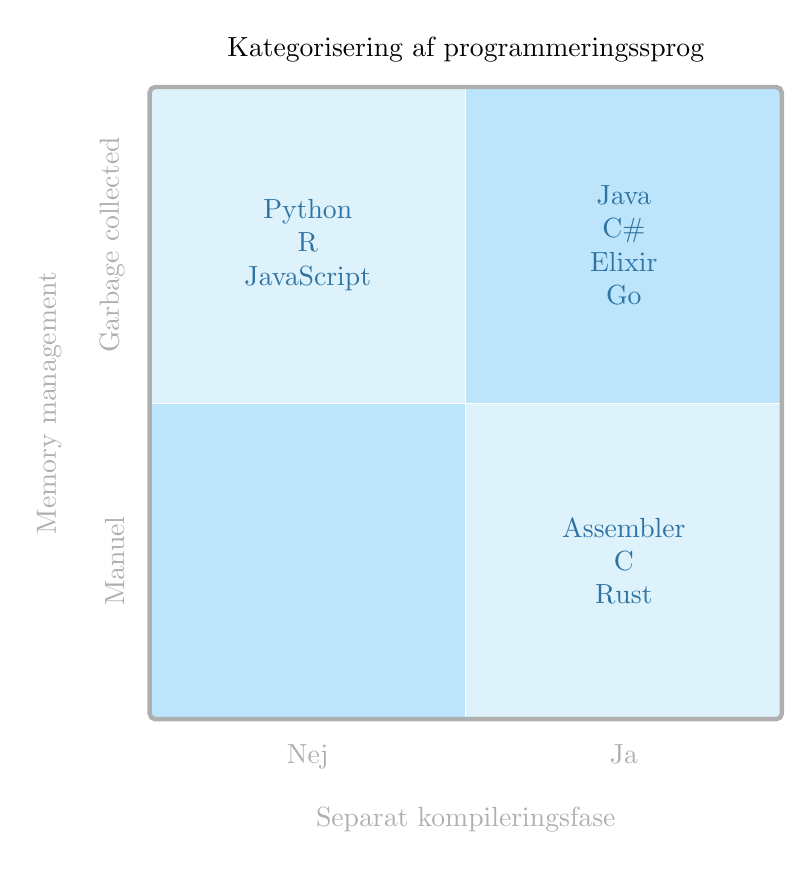
\begin{tikzpicture}[squares/.style={align=center, text width=3cm, text=bluetext, minimum width=4cm, minimum height=4cm}]

    \node[squares,fill=lightblue] (A) at (0,0) {Python\\R\\JavaScript};
    \node[squares,fill=darkblue,anchor=west] (B) at (A.east) {Java\\C\#\\Elixir\\Go};
    \node[squares,fill=darkblue,anchor=north] (C) at (A.south){};
    \node[squares,fill=lightblue,anchor=north] (D) at (B.south) {Assembler\\C\\Rust};
    \node[inner sep=0pt,draw=grey,ultra thick,rounded corners=2pt,fit=(A)(B)(C)(D)] {}; 

    \node[align=center,anchor=south,yshift=2mm] at (A.north east) {Kategorisering af programmeringssprog};
    \node[anchor=east,text=grey,xshift=-2mm] at (A.west) {\rotatebox{90}{Garbage collected}};
    \node[anchor=east,text=grey,xshift=-1cm,align=right] at (A.south west) {\rotatebox{90}{Memory management}};
    \node[anchor=east,text=grey,xshift=-2mm] at (C.west) {\rotatebox{90}{Manuel}};
    \node[anchor=north,text=grey,yshift=-2mm] at (C.south) {Nej};
    \node[anchor=north,text=grey,yshift=-1cm] at (C.south east) {Separat kompileringsfase};
    \node[anchor=north,text=grey,yshift=-2mm] at (D.south) {Ja};
\end{tikzpicture}


\section{Parsing}

% file content
Indholdet af en fil er en sekvens af bytes, altså værdier der hver især har én af 256 mulige værdier. Når vi skriver tekst fortolkes disse bytes som tegn og de programmer vi bruger til at åbne sådanne filer vælger at tegne hvert tegn til højre for det forrige. Ved linjebrud -- der repræsenteres ved en bestemt sekvens af tegn -- flyttes den horisontale position helt til venstre og der rykkes en linjehøjde nedaf. Nogle programmer bryder linjer der er for brede til ens skærm. Men det er sådan set det. En sådan tekstfil indeholder ikke nogen information om font eller tekststørrelse. Ønsker man at gemme sådanne informationer er man nødt til at introducere et \textsl{filformat}, der \textsl{koder} sådanne informationer ved sårlige opmærkninger. Men det er ikke relevant for filer der indeholder kode.

% human interpretation
Filer der indeholder kode er rå tekstfiler: En sekvens af tegn med linjebrud. Som programmører manipulerer vi disse filer igennem en teksteditor, der oftest -- ud over selve visningen af disse tegn -- vælger at farvekode udvalgte delsekvenser for at gøre teksten mere overskuelig for mennesker. Disse farver repræsenterer dog en \textsl{fortolkning} som værktøjet bruger til at berige koden. På samme måde er der nogen sådanne editorer der nummererer linjerne, fremhæver en aktuelle linje og markerer matchende parenteser.

% machine interpretation
Den tekst disse filer indeholder kaldes for \textsl{programkode} (eller blot \textsl{kode}), og vi ændrer i den på nogenlunde samme måde som vi ændrede i en dansk stil. Men når vi beder computeren om at køre noget med vores programkode så ser den filen på en anden måde. Indholdet er naturligvis det samme, men \textsl{fortolkningen} er anderledes: På baggrund af nogle regler opbygger computeren en træstruktur af programmet.

% TODO: træstruktur

\subsection{Regler}

% https://homepage.ruhr-uni-bochum.de/jan.holthuis/posts/using-the-latex-rail-package

\subsection{Parsetræer}

% https://tex.stackexchange.com/questions/111564/create-a-syntax-tree-with-latex

\chapter{Programmeringssprog}
\label{sec:lang}

\begin{inspiration}{Larry Wall}
Computer language design is just like a stroll in the park. Jurassic Park, that is.
\end{inspiration}

% inspiration: https://tex.stackexchange.com/questions/309425/how-is-it-possible-to-make-a-magic-quadrant
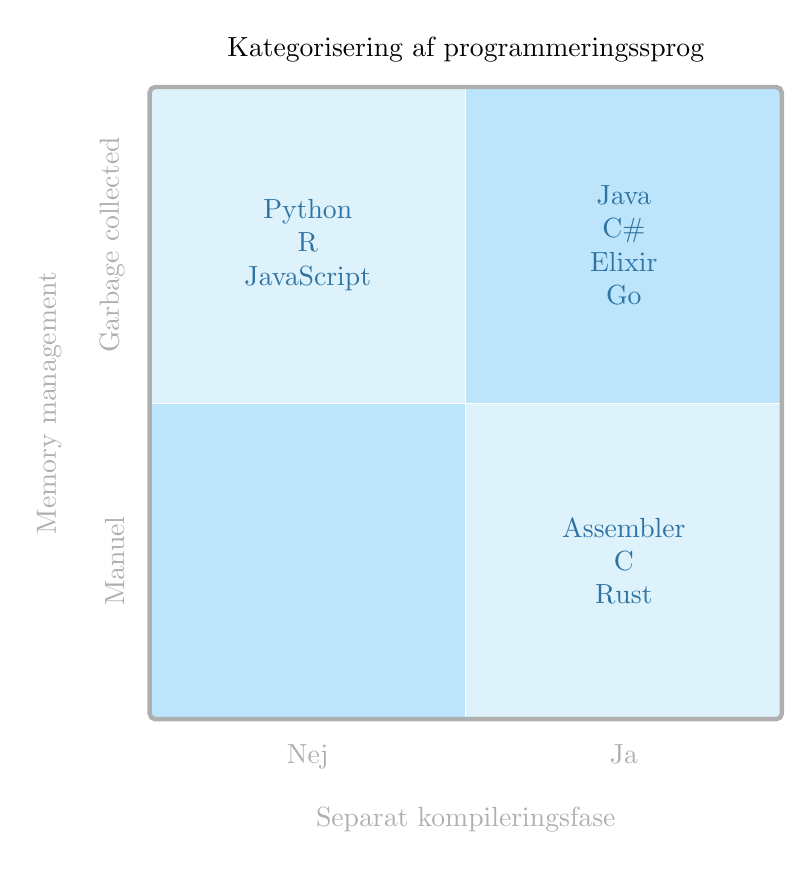
\begin{tikzpicture}[squares/.style={align=center, text width=3cm, text=bluetext, minimum width=4cm, minimum height=4cm}]

    \node[squares,fill=lightblue] (A) at (0,0) {Python\\R\\JavaScript};
    \node[squares,fill=darkblue,anchor=west] (B) at (A.east) {Java\\C\#\\Elixir\\Go};
    \node[squares,fill=darkblue,anchor=north] (C) at (A.south){};
    \node[squares,fill=lightblue,anchor=north] (D) at (B.south) {Assembler\\C\\Rust};
    \node[inner sep=0pt,draw=grey,ultra thick,rounded corners=2pt,fit=(A)(B)(C)(D)] {}; 

    \node[align=center,anchor=south,yshift=2mm] at (A.north east) {Kategorisering af programmeringssprog};
    \node[anchor=east,text=grey,xshift=-2mm] at (A.west) {\rotatebox{90}{Garbage collected}};
    \node[anchor=east,text=grey,xshift=-1cm,align=right] at (A.south west) {\rotatebox{90}{Memory management}};
    \node[anchor=east,text=grey,xshift=-2mm] at (C.west) {\rotatebox{90}{Manuel}};
    \node[anchor=north,text=grey,yshift=-2mm] at (C.south) {Nej};
    \node[anchor=north,text=grey,yshift=-1cm] at (C.south east) {Separat kompileringsfase};
    \node[anchor=north,text=grey,yshift=-2mm] at (D.south) {Ja};
\end{tikzpicture}


\section{Parsing}

% file content
Indholdet af en fil er en sekvens af bytes, altså værdier der hver især har én af 256 mulige værdier. Når vi skriver tekst fortolkes disse bytes som tegn og de programmer vi bruger til at åbne sådanne filer vælger at tegne hvert tegn til højre for det forrige. Ved linjebrud -- der repræsenteres ved en bestemt sekvens af tegn -- flyttes den horisontale position helt til venstre og der rykkes en linjehøjde nedaf. Nogle programmer bryder linjer der er for brede til ens skærm. Men det er sådan set det. En sådan tekstfil indeholder ikke nogen information om font eller tekststørrelse. Ønsker man at gemme sådanne informationer er man nødt til at introducere et \textsl{filformat}, der \textsl{koder} sådanne informationer ved sårlige opmærkninger. Men det er ikke relevant for filer der indeholder kode.

% human interpretation
Filer der indeholder kode er rå tekstfiler: En sekvens af tegn med linjebrud. Som programmører manipulerer vi disse filer igennem en teksteditor, der oftest -- ud over selve visningen af disse tegn -- vælger at farvekode udvalgte delsekvenser for at gøre teksten mere overskuelig for mennesker. Disse farver repræsenterer dog en \textsl{fortolkning} som værktøjet bruger til at berige koden. På samme måde er der nogen sådanne editorer der nummererer linjerne, fremhæver en aktuelle linje og markerer matchende parenteser.

% machine interpretation
Den tekst disse filer indeholder kaldes for \textsl{programkode} (eller blot \textsl{kode}), og vi ændrer i den på nogenlunde samme måde som vi ændrede i en dansk stil. Men når vi beder computeren om at køre noget med vores programkode så ser den filen på en anden måde. Indholdet er naturligvis det samme, men \textsl{fortolkningen} er anderledes: På baggrund af nogle regler opbygger computeren en træstruktur af programmet.

% TODO: træstruktur

\subsection{Regler}

% https://homepage.ruhr-uni-bochum.de/jan.holthuis/posts/using-the-latex-rail-package

\subsection{Parsetræer}

% https://tex.stackexchange.com/questions/111564/create-a-syntax-tree-with-latex


\end{document}

